\documentclass[showpacs,showkeys,10pt,onecolumn,superscriptaddress,notitlepage]{revtex4-1}

\usepackage[ansinew]{inputenc}
\usepackage[T1]{fontenc}

\usepackage{amsmath,amsthm,amssymb,amscd}
\usepackage{bbm}
\usepackage{mathtools}
\usepackage{hyperref}

\newcommand{\Epi}{\affiliation{Department of Epileptology, University of Bonn, Venusberg Campus 1, 53127~Bonn, Germany}}
\newcommand{\HISKP}{\affiliation{Helmholtz Institute for Radiation and Nuclear Physics, University of Bonn, Nussallee~14--16, 53115~Bonn, Germany}}
\newcommand{\IZKS}{\affiliation {Interdisciplinary Centre for Complex Systems, University of Bonn, Br\"uhler Stra\ss{}e~7, 53175~Bonn, Germany}}
\newcommand{\ICBM}{\affiliation {Department of physics, Sharif University of Technology, 11365-9161, Tehran, Iran}}
\newcommand{\RNS}{\affiliation{Institute of Physics and ForWind, Carl von Ossietzky University of Oldenburg,\\ Carl-von-Ossietzky-Stra\ss{}e~9--11, 26111~Oldenburg, Germany}}
\newcommand{\THP}{\affiliation{Institute for Theoretical Physics, University of Cologne, 50937 K\"oln, Germany}}
\newcommand{\FZJ}{\affiliation{Forschungszentrum J\"ulich, Institute for Energy and Climate Research - Systems Analysis and Technology Evaluation (IEK-STE), 52428 J\"ulich, Germany}}
\newcommand{\Bethe}{\affiliation{Physikalisches Institut and Bethe Center for Theoretical Physics, Universit\"at Bonn, Nussallee 12, 53115 Bonn, Germany}}


\frenchspacing

\begin{abstract}
    This preprint presents an open-source Python library to calculate Kramers--Moyal coefficients, for any desired order, for one- an two-dimensional stochastic processes.
    The library relies on a kernel-based regression to obtain accurate results for data with a low number of data points, while allowing a straightforward way to calculate the Kramers--Moyal coefficients of a stochastic process at any desired order.
    The library is a standalone python package dependent only on \texttt{numpy} and \texttt{scipy}, and is ready for research application. 
\end{abstract}

\begin{document}

\title{Python KM: Higher-order Kramers--Moyal coefficients for one- and two-dimensional stochastic processes} 


\author{Leonardo~Rydin~Gorj\~ao}
\email[Electronic mail: ]{l.rydin.gorjao@fz-juelich.de}
\Epi \HISKP \THP \FZJ 

\author{Francisco Meirinhos}
\Bethe

\keywords{Kramers--Moyal coefficents, stochastic processes, jump-diffusion processes, Fokker--Planck equation, Python}

\maketitle

\textbf{Library available at}:  \texttt{\href{https://github.com/LRydin/KramersMoyal}{github.com/LRydin/KramersMoyal}}

\section{Summary}

A general problem for evaluating stochastic processes is the retrieval of the Kramers--Moyal coefficients $\mathcal{M}$ from data or time-series.
The Kramers--Moyal coefficients are derived from an expansion of the master equation that describes a particular stochastic process.

Given a set of continuous and stationary data, i.e., ergodic or quasi-stationary stochastic data, the extensive literature of stochastic processes awards a set of measures, such as the Kramers--Moyal coefficients or the conditional moments, whcih link stochastic processes to a probabilistic description of the process or of the family of processes \cite{Risken}. Most commonly known is the set the partial differential equations, the Fokker--Planck equations, derived from the master equation as a lower-order truncation of the stochastic process.
Of particular relevance is the growing evidence that lower-order stochastic processes do not seem to accurately describe phenomena seen in data, which necessitates the study of higher-order processes, and therefore a way to efficiently uncover the higher-order Kramers--Moyal coefficients from data \cite{Tabar}.
Moreover, the presence of discontinuous jumps in data has gained attention through jump-diffusion modelling, which has found applications in wind- and solar-power systems \cite{Anvari} and finance \cite{Sahalia}.

The most straightforward approach is to perform a histogram-based regression to evaluate the conditional moments of the system at hand.
Such an approach is conventional and requires the most commonly used packages in Python (i.e., \texttt{numpy},  \texttt{scipy}, or \texttt{pandas}), and is directly embodied in MATLAB, Julia, or R, usually under the name of \texttt{hist} or \texttt{histogram}.
This library is based on a kernel-based regression, which allows for more robust results given both a wider range of possible kernel shapes to perform the calculation, as well as retrieving the results in a non-binned coordinate space, unlike histogram regressions \cite{Silverman}.

The package presented here comprises a manifold of options: A general open-source toolbox for the calculation of Kramers--Moyal coefficients in one and two dimensions, for any desired order, with a variety of different kernels, as well as the possibility of extending the code for three or more dimensions.

\section{Mathematics}

The probability that an $n$-dimensional state variable $\boldsymbol{x}'(t)\in\mathbb{R}^n$ is observed at position $\boldsymbol{x}$ is given by the conditional probability of the previous (or future) states of the system \cite{Risken}.
This probabilistic description takes the form
\begin{equation}
\mathcal{M}^{[\ell]}(\boldsymbol{x},t)=\int  dx'(\boldsymbol{x}(t)'-\boldsymbol{x}(t))^\ell W(\boldsymbol{x}'|\boldsymbol{x}),
\end{equation}
with $W(\boldsymbol{x}'|\boldsymbol{x})$ the transition probability rate.

The exact evaluation of the Kramers--Moyal coefficients for discrete or discretised datasets $\boldsymbol{y}(t)$---any human measure of a process is discrete, as well as any computer generated data---is bounded by the timewise limit imposed.
Taking as an example a two-dimensional case, that one can obtain numerically with this library, with $\boldsymbol{x}(t)=(x_1(t),x_2(t))\in\mathbb{R}^{2}$, the Kramers--Moyal coefficients $\mathcal{M}^{[\ell, m]}\in\mathbb{R}^{2}$ take the form
\begin{equation}
\begin{aligned}
&\mathcal{M}^{[\ell, m]}(x_1,x_2)=\lim_{\Delta t\to 0}\!\frac{1}{\Delta t}\int \mathrm{d} y_1 \mathrm{d} y_2 (y_1(t\!+\!\Delta t)\!-\!y_1(t))^\ell(y_2(t\!+\!\Delta t)\!-y_2(t))^m \cdot \\
& \qquad \qquad \qquad \qquad \qquad \qquad \qquad P(y_1,y_2; t\!+\!\Delta t|y_1,y_2 ; t)|_{y_1(t)=x_1, y_2(t)=x_2},
\end{aligned}
\end{equation}
at a certain measure point $(x_1,x_2)$. The Kramers--Moyal coefficients $\mathcal{M}^{[\ell, m]}(x_1,x_2)$ are obtained from a two-dimensional time-series $(y_1(t),y_2(t))$.

Theoretically, $\Delta t$ should take the limiting case of $\Delta t \to 0$, but the restriction of any measuring or storing device---or the nature of the observables themselves---permits only time-sampled or discrete recordings.
The relevance and importance of adequate time-sampling was extensively studied and discussed in \cite{Lehnertz}.
In the limiting case where $\Delta t$ is equivalent to the sampling rate of the data, the Kramers--Moyal coefficients take the form
\begin{equation}
\begin{aligned}
\mathcal{M}^{[\ell, m]}(x_1, x_2) = \frac{1}{\Delta t} \langle \Delta y_1^{\ell} \Delta y_2^{m} |_{y_1(t)=x_1, y_2(t)=x_2}\rangle,~\mathrm{with}~\Delta y_i =  y_i(t+ \Delta t) - y_i(t).
\end{aligned}
\end{equation}

The order of the Kramers--Moyal coefficients is given here by the superscript $\ell$ and $m$.
For such measure of the Kramers--Moyal coefficients, i.e., a probabilistic measure, a probabilistic space exists, assigned to the process, stemming from the master equation describing the family of such processes.
The conventional procedure is to utilise a histogram regression of the observed process and retrieve, via approximation or fitting, the Kramers--Moyal coefficient.
The choice of a histogram measure for the Kramers--Moyal coefficient results in an acceptable measure of the probability density functions of the process but requires a new mathematical space (a distribution space).
The usage of a kernel approach, implemented in this library, permits an identical overview without the necessity of a new (discretised) distribution space, given that the equivalent space of the observable can be taken.

Like the histogram approach for the measure of the Kramers--Moyal coefficients, each single measure of the observable $\boldsymbol{y}(t)$ is averaged, with a designed weight, into the distribution space.
The standing difference, in comparison to the histogram approach, is the riddance of a (discrete) binning system.
All points are averaged, in a weighted fashion, into the distribution space---aiding specially in cases where the number of point in a dataset is small---and awarding a continuous measurable space (easier for fitting, for example) \cite{Lamouroux}.

\begin{figure}[h]
    \centering
    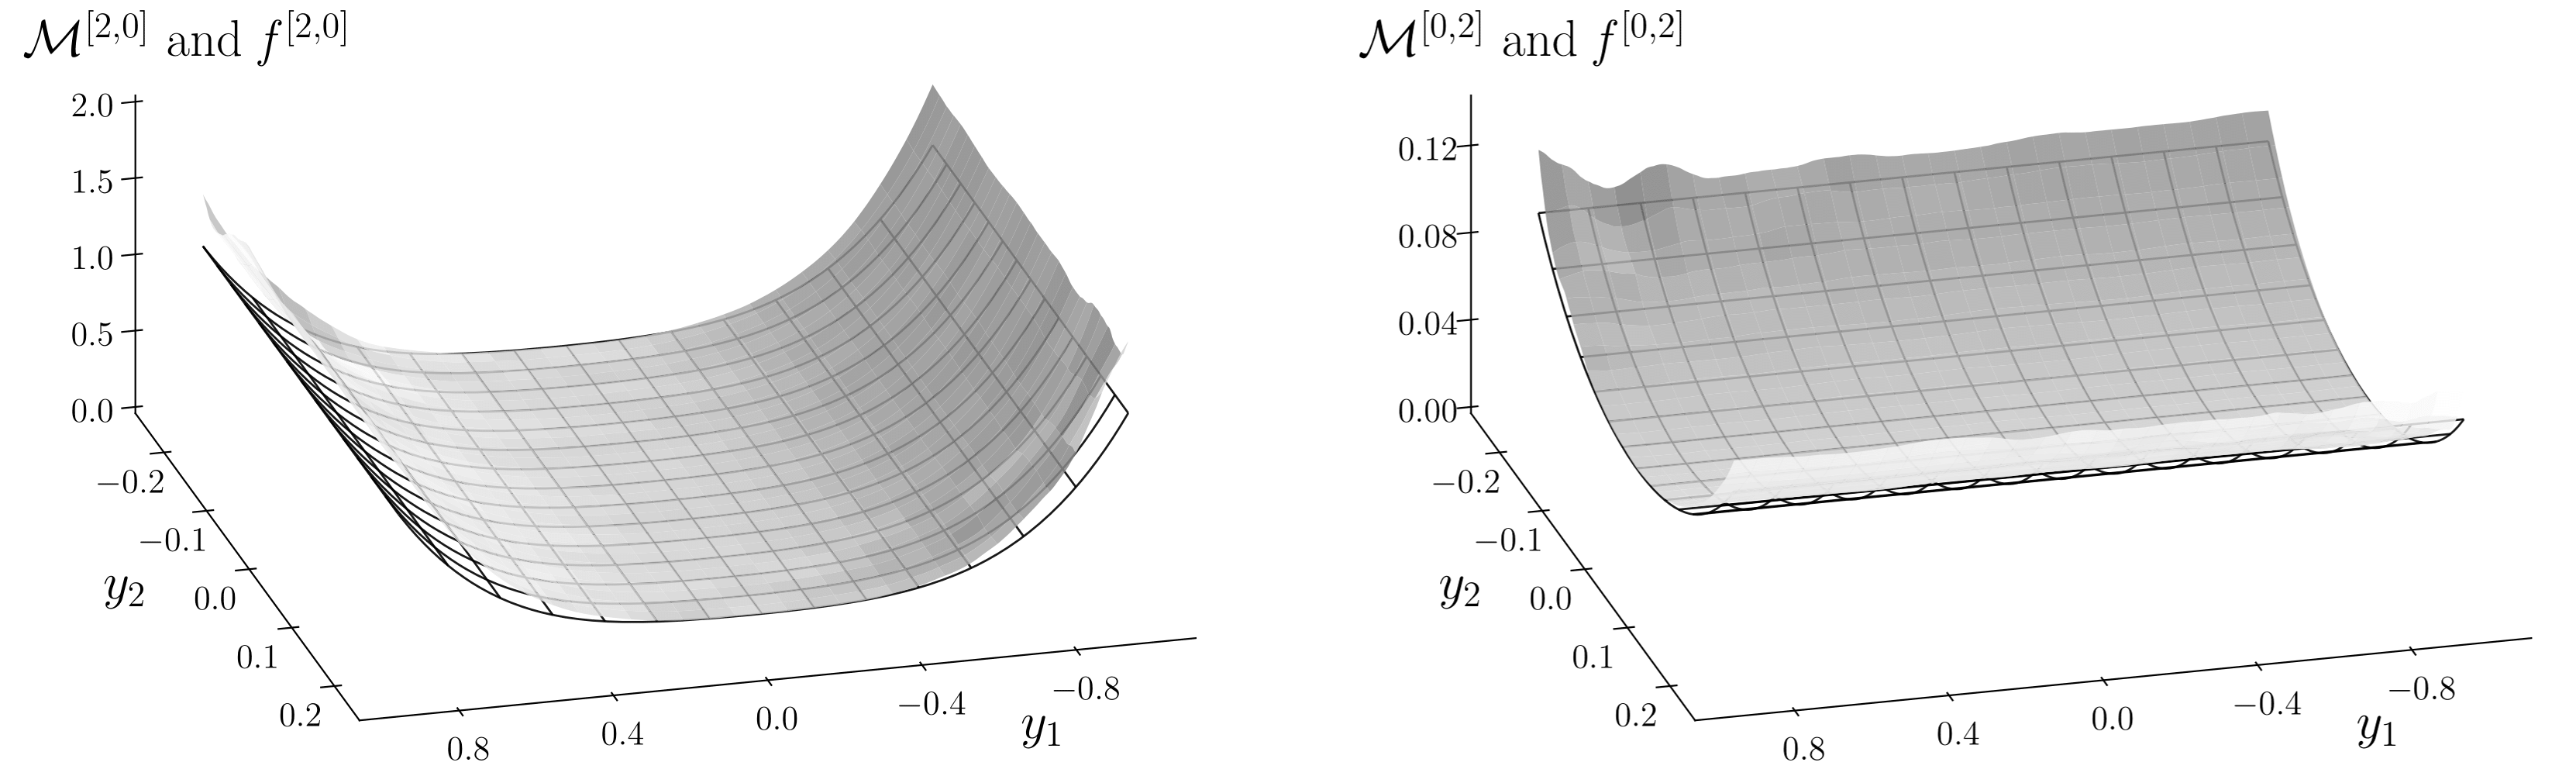
\includegraphics[width=0.9\linewidth]{figure.png}
    \caption{Two exemplary two-dimensional Kramers--Moyal coefficients for a stochastic process were calculated with a package using a $n\times n = 440\times 440$ array. Plotted as well are the theoretical surfaces according to \cite{Anvari}. An asymmetric two-dimensional Epanechnikov kernel was employed \cite{Epanechnikov,Lamouroux}. The data was generated using \texttt{JiTCSSD} \cite{Ansmann}.}
\end{figure}

\section{Library}
The presented library is comprised of two separate blocks, \texttt{kernels} and \texttt{km}, and is a standalone package for a non-parametric retrieval of Kramers--Moyal coefficients, solely dependent on \texttt{numpy} and \texttt{scipy}. The sub-module \texttt{kernels} comprises the kernels for the kernel-based estimation, similarly available in \texttt{sklearn}, and \texttt{km} performs the desired Kramers--Moyal calculations to any desired power \cite{scikitlearn}.

\section{Declaration of interest}
This package is openly available on GitHub at: \texttt{\href{https://github.com/LRydin/KramersMoyal}{github.com/LRydin/KramersMoyal}} and is still in an experimental stage. Comments, remarks, improvements, and reviews are appreciated.
This article will be submitted to \textit{The Journal of Open Source Software} at: \texttt{\href{https://joss.theoj.org}{joss.theoj.org}} [ISSN: 2475-9066, OCLC number: 971252162].
The Python library will be maintained always in open-source structure.
The authors declare no conflict of interest.

\section{Acknowledgements}
L. R. G. thanks Klaus Lehnertz and M. Reza Rahimi Tabar for all the help in understanding stochastic processes and developing this package, Dirk Witthaut for the support during the process of writing and reviewing, Gerrit Ansmann for the help in understanding python's intricacies, and Marieke Helmich for the text reviews.
L. R. G. gratefully acknowledges support by the Helmholtz Association, via the joint initiative \emph{Energy System 2050 - A Contribution of the Research Field Energy}, and the grant No. VH-NG-1025 and F. M. gratefully acknowledges the fund, in part, by the Deutsche Forschungsgemeinschaft (DFG, German Research Foundation), project number 277625399 - CRC 185.

\bibliography{bib}

\end{document}


